%%%%%%%%%%%%%%%%%%%%%%%%%%%%%%%%%%%%%%%%%%%%%%%%%%%%%%%%%%%%%%%%%%
%%%%%%%% CPSC 68 SPRING 2017 EXAMPLE REPORT %%%%%%%%%%%%%%%%%%%%%%%%
%%%%%%%% This template is modified from ICML 2014 %%%%%%%%%%%%%%%%
%%%%%%%%%%%%%%%%%%%%%%%%%%%%%%%%%%%%%%%%%%%%%%%%%%%%%%%%%%%%%%%%%%

\documentclass{article}

%include any external packages here.  This is similar to loading a
%library in python or C++

% use Times
\usepackage{times}
% For figures
\usepackage{graphicx}
\usepackage{subfigure}

% For citations
\usepackage{natbib}

% For algorithms and pseudocode
\usepackage{algorithm}
\usepackage{algorithmic}

%Adds hyperlinks to your citations automatically
\usepackage{hyperref}

% Packages hyperref and algorithmic misbehave sometimes.  We can fix
% this with the following command.
\newcommand{\theHalgorithm}{\arabic{algorithm}}

\usepackage[accepted]{icml2014}


% If your title is long (below), use this command to also provide
% short version.  This will go on the top of every page
\icmltitlerunning{Final Report}

\begin{document}

\twocolumn[ %use two column if you need a text to span across the whole page
\icmltitle{Pill image segmentation }

\icmlauthor{Alison Rosenzweig}{arosenz1@swarthmore.edu}
\icmlauthor{Emma Remy}{eremy1@swarthmore.edu}

\vskip 0.3in
]

\begin{abstract}
In 2016, the National Library of Medicine (NLM) hosted the Pill Image Recognition Challenge to accurately identify pills based on smartphone-quality images \cite{PIR}. This problem is particularly pertinent for medical professionals and their patients who need to regularly identify pills by sight. Unfortunately, it is also programmatically difficult, due to irregularities in the images like complex backgrounds and variations in lighting and color; to mitigate these problems, we segment the images to separate pills and backgrounds. We compare several algorithms for image segmentation, including simple thresholding, Watershed, and thresholding on the distance from the median color in both RGB and HSV color spaces. While no method gave consistent results for lower-quality images, we found thresholding on distance from the median is extremely effective for segmenting reference-quality images.
\end{abstract}

\section{Introduction}
\label{introduction}

The NLM Pill Image Recognition Challenge (NLM PIR) from 2016 asked for an algorithm to 
map customer images of pills to a set of reference images in order to identify a pill \cite{PIR}. This problem involves first identifying the pills in the images, and then comparing pills and pill features across images to identify the correct pill. We focus on image segmentation, comparing simple thresholding, Watershed, and thresholding on the distance from the median color in both the RGB and HSV color spaces. Thresholding on distance from median consistently and accurately segmented reference images, although we found no method very effective in consistently segmenting pills from lower-quality images.

The NLM PIR provided images of 1,000 different pills, two each of reference quality and five of customer-quality. The reference quality images are close-up, well-lit images of individual pills with consistent, medium-gray backgrounds, such as Figure \ref{fig:ref-two-color}. The customer-quality images are taken with smartphone cameras and include harsh shadows, differently colored light, blurriness, and backgrounds varying in color and pattern, such as Figure \ref{fig:cust-weird-bg}. The purpose of the NLM PIR is to reliably identify a pill from even a low-quality image of this kind.

% an example of a reference image
\begin{figure}
    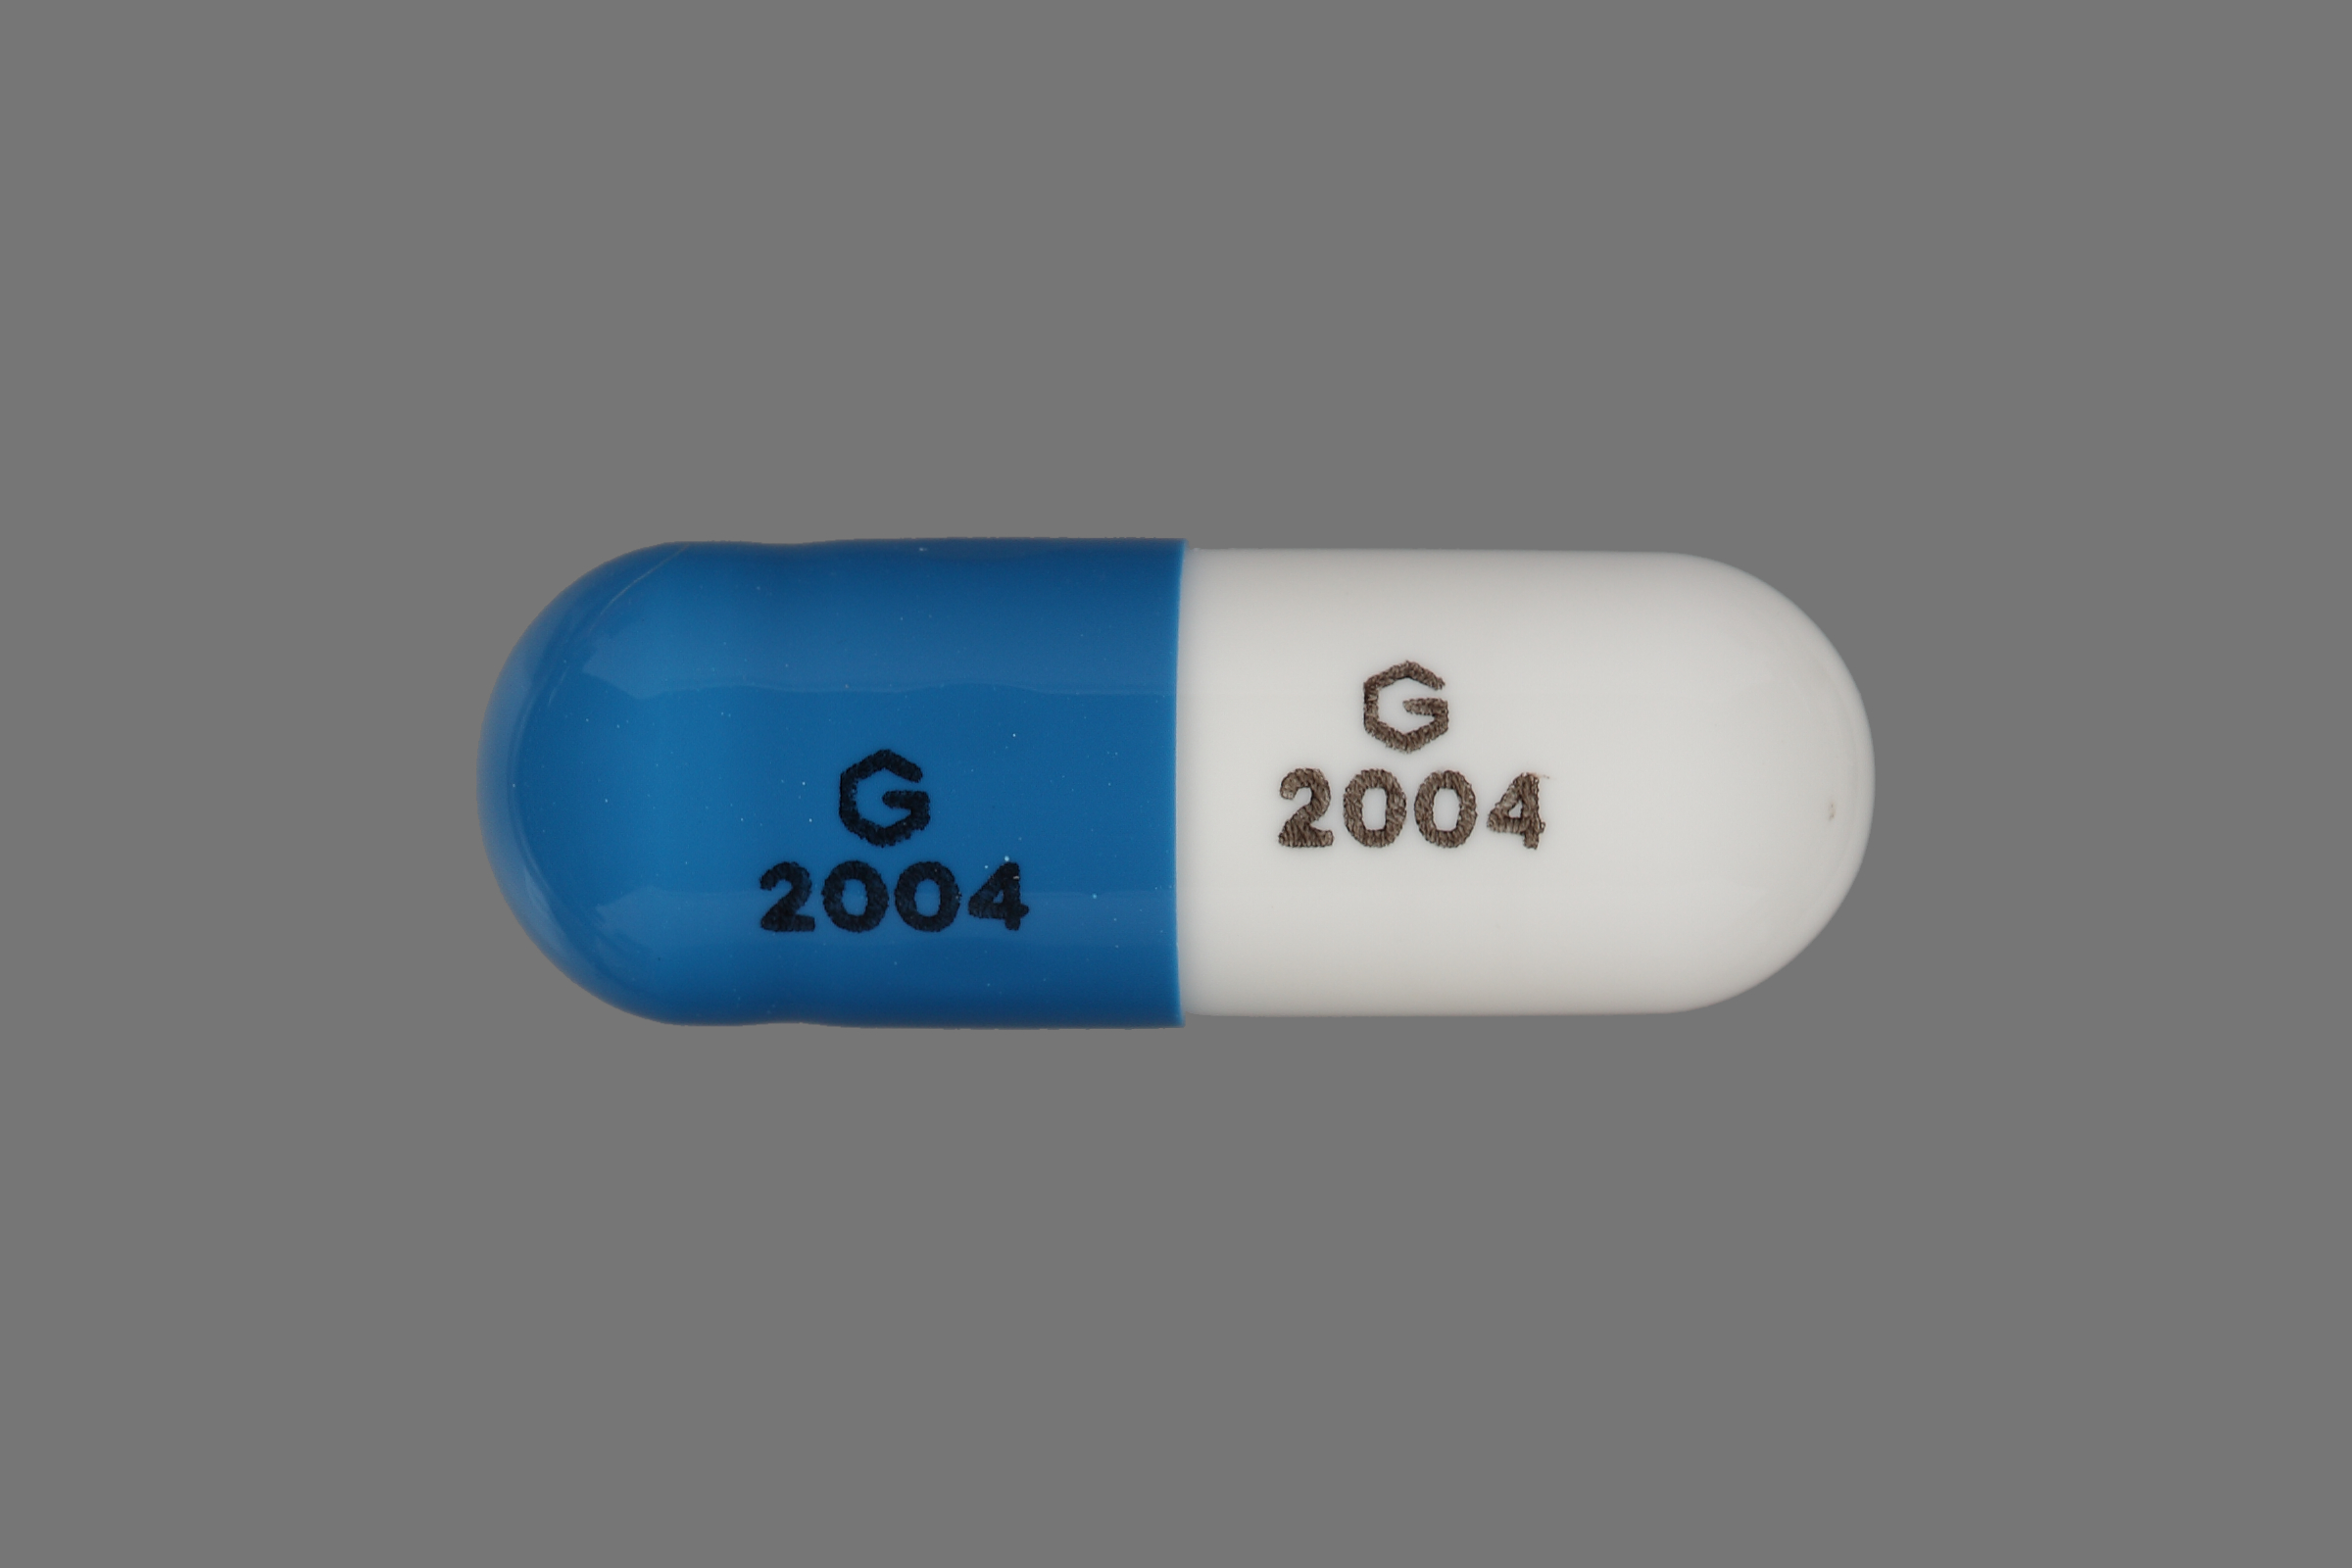
\includegraphics[width=\linewidth]{images/ref_two_color.jpg}
    \caption{A reference image for a two-tone pill.}
    \label{fig:ref-two-color}
\end{figure}

% an example of a customer-quality image
\begin{figure}
    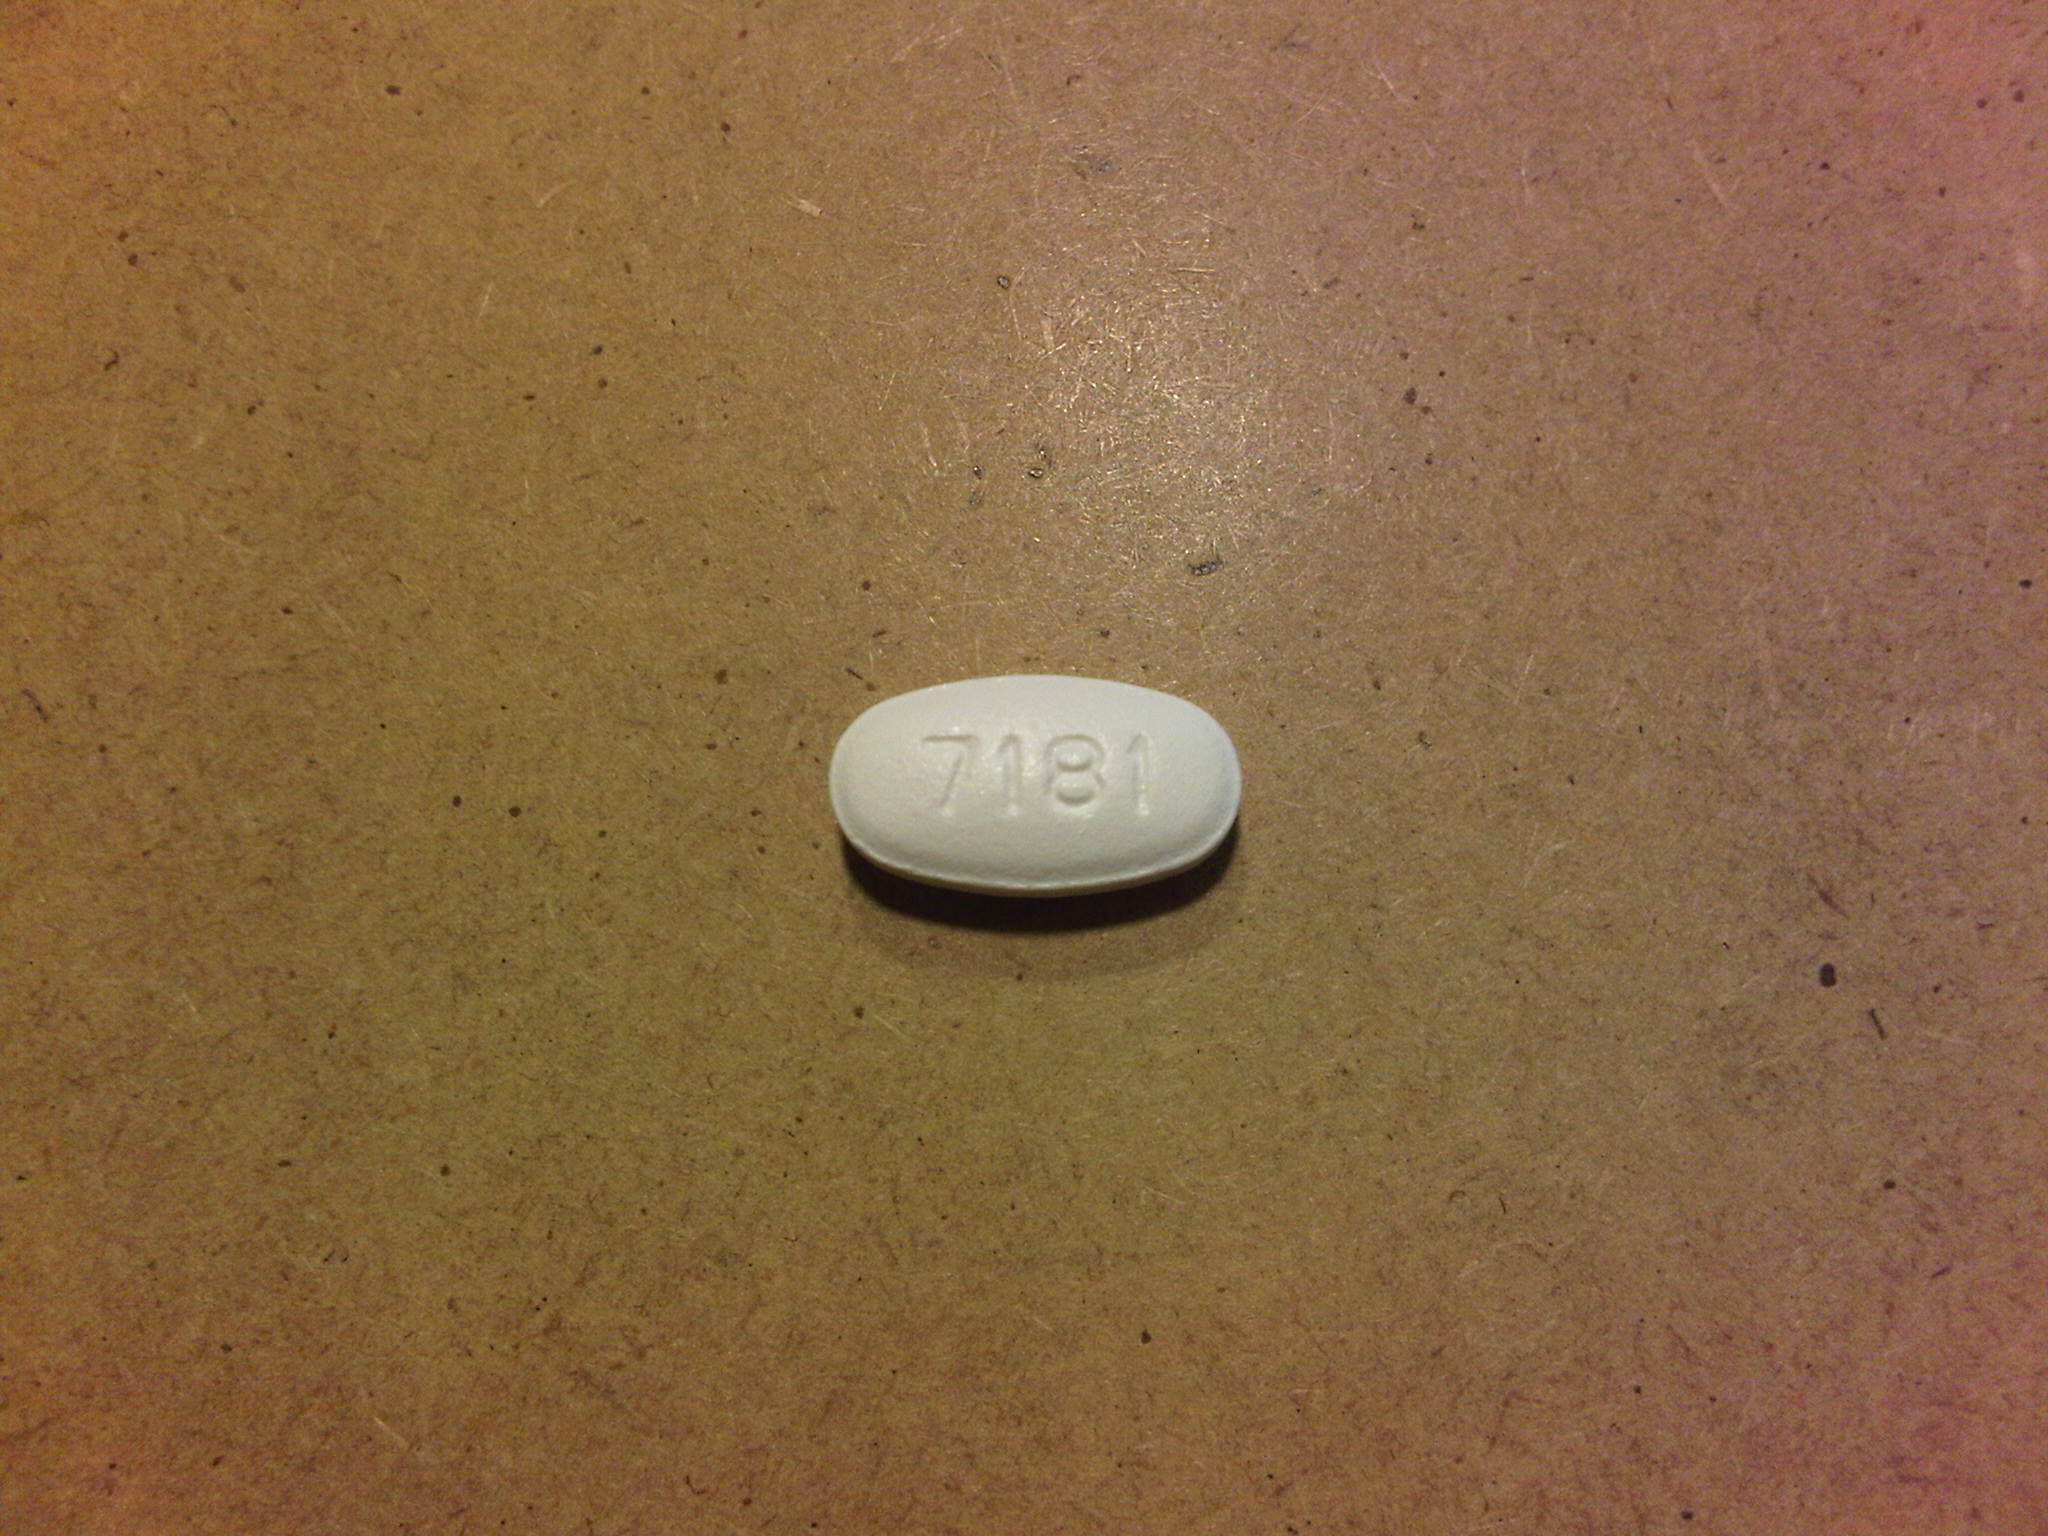
\includegraphics[width=\linewidth]{images/cust_weird_bg.jpg}
    \caption{A customer-quality image with a patterned background.}
    \label{fig:cust-weird-bg}
\end{figure}

This kind of medication identification is extremely useful in many contexts, particularly for medical officials and their patients. Doctors and pharmacists regularly handle many different pills, so having a tool to quickly and accurately identify pills with just a smartphone allows can increase efficiency and help prevent mistakes. It may also be useful for patients taking several medications who have trouble keeping track of their pills, especially for those patients who are visually-impaired or otherwise unable to easily verify their pills without assistance. Mixing up medications can have serious consequences which the NLM PIR seeks to prevent by allowing for easier pill identification.

Unfortunately, the variation in the customer-quality images makes this task difficult. The customer quality images are often poorly lit with harsh shadows, color variation, blurriness, and patterned backgrounds. Additionally, some pills are very similar in color to the background (e.g. a white pill on a white background) and some capsule-style pills are multiple colors. All of these factors make it hard to reliably identify salient characteristics like pill color or characters printed or inscribed on the pill from the customer quality images, complicating general identification.

In order to eliminate some of the variation between images, we focus on segmenting the images to separate pills from their backgrounds. We compare several methods of segmentation: simple thresholding, the Watershed algorithm, thresholding on the distance from the median color, and k-means clustering; we also consider different color spaces for each method. We evaluate the effectiveness of each segmentation method using Dice’s coefficient, and find that no method is effective for segmenting the customer-quality images, but thresholding on distance from the median is extremely effective for segmenting reference-quality images.

Overall, we are not able to effectively segment pills from customer-quality images. We can segment reference-quality images, and we are able to segment some particular customer-quality images. In the future, we will combine and explore new methods of segmentation and classification, perhaps utilizing a neural network or other machine learning techniques.

\section{Related works}
\label{related}

The NLM PIR Challenge was proposed because, at the time, there were no any good solution to the problem of pill identification from low-quality images. The winners of the challenge produced a working tool to identify pills from smartphone images, but have not published their results \cite{fox}. There is plenty of work being done in image segmentation that we intend to build off of, as well as work in pill identification from features rather than images \cite{semantic-segmentation}. Additionally, while none of the winners of the NLM PIR Challenge have yet published their results, researchers Ushizima et al. published their contribution to the project \cite{ushizima}. 

The NLM has done work in the past toward pill identification; the NLM Pillbox accurately identifies pills based on salient features like color and imprint (the words or numbers stamped on or engraved in the pill)\cite{pillbox}. The Pillbox is accurate and freely available for public use, but not convenient for rapid identification of many pills. It also is hard to use for patients or medical professionals with visual impairments. The existence and success of this tool point to a potential technique for identifying pills by images: if we could extract features like color, shape, and imprint from the images, we would easily be able to identify these pills. However, this strategy is far from simple.  It would rely on complex (and sometimes unreliable) computer vision techniques for segmenting the pill, correcting the color and shadows, identifying and reading imprints, etc. 

While none of the winners of the NLM PIR Challenge have published results, Ushizima et al. published their use of the NLM PIR data to gather feature data from reference images \cite{ushizima}. They successfully extracted shape and size data from the reference images. From this, they clustered the pills to establish that the NLM PIR Challenge reference image dataset reflects the true distribution of pill shapes and provided a potential starting point for anyone competing in the NLM PIR Challenge. Ushizima et al. use edge-detection and sharpening techniques to segment the reference images, noting challenges in thresholding-based techniques. We aim to return to these simpler color- and thresholding-based techniques and quantitatively evaluate their success on reference and customer-quality images. 

Lots of promising work exists in pill identification by human-extracted features as well as early work in the segmentation of pill images. However, reliably segmenting or extracting useful features from lower quality pill images is still an open and important area of research for developing a reliable image-based pill identification tool.

\section{Approaches}
\label{approaches}

\subsection{Simple thresholding}

Thresholding turns grayscale (single-channel) images into black and white (binary) images by rounding values above a given threshold $\tau$ to the maximum value and values below $\tau$ to the minimum value \cite{cv-textbook}. 

We use simple thresholding, with images in both RGB and HSV space, to create binary masks. In RGB space we threshold on the standard grayscale pixel values. In HSV space we threshold within the hue channel (i.e. segmenting based on color, not brightness or saturation). 

We use two types of thresholds: a binary inverse threshold and an Otsu threshold. The Otsu threshold iterates over a range of threshold values and chooses the one that results in the least spread within the two groups, where the two groups are the clusters of pixel values that fall above and below the threshold. The binary inverse threshold sets pixels below the given threshold to 1 and the pixels above the threshold to 0. Using these two together (in OpenCV) has inversing effect of the binary inverse threshold but disregards the given threshold in favor of the optimization used by the Otsu threshold \cite{cv-textbook}. 

\subsection{Distance to average}

Simple thresholding works on a single channel in an image. It is thresholding either based on just the overall pixel intensity (RGB space) or on the hue of the pixel (HSV space). However, the portions of the image that differ most in these dimensions may not be the pill. Other features of customer quality images in particular may impact the results (e.g. harsh shadows or differently colored speckles on a background). Additionally, it is inconsistent if the pill in an image will tend to have higher or lower values in the single-channel images than the background -- there may be a light-colored pill on a black surface or vice versa. We therefore threshold the image based on the distance from each pixel to the \textit{average} pixel in that image, with several variations: we use both the mean and median pixel values in both the HSV and RGB color spaces. 

In order to execute this, we calculate the mean or median of the image. We then create an image where every pixel value is equal to the distance between that pixel in the original image and the mean or median pixel value. With $\bar{x}$ equal to the chosen representative pixel value (the mean or median of the image), the pixel at position $(i, j)$ in the image takes on the value 
\small
$$||img[i, j] - \bar{x}|| =$$
$$\sqrt{(img[i, j]_1 - \bar{x}_1)^2+(img[i, j]_2 - \bar{x}_2)^2 + (img[i, j]_3 - \bar{x}_3)^2}$$
\normalsize
where $1$, $2$, and $3$ denote the 3 image channels (in either RGB or HSV space). To create a mask from this image, we apply a binary threshold to this distance image. Finally, we apply our morphological operations method (including smoothing and re-thresholding), producing a smoothed binary mask. 

\subsection{Watershed algorithm}

The Watershed Algorithm is a commonly used computer vision technique for segmenting single-channel images \cite{semantic-segmentation}, common especially for use with medical images \cite{medical}. It works by treating images as topographies where the pixel intensities correspond to elevations \cite{watershed-legit}. Much of the advantage of the watershed algorithm lies in its ability to separately identify adjacent regions (e.g. coins touching on a flat surface) where traditional thresholding techniques would, at best, be able to segment all the touching coins as contiguous region. 

The Watershed Algorithm segments regions differently than simple thresholding. Rather than looking at each pixel individually, the Watershed algorithm starts at identified key points or marks and then moves outwards from those analogously to a graph-filling algorithm. In the case of the implementation we use, the key points are determined heuristically by choosing local minima of pixel values in the grayscale image. 

Notably, the Watershed Algorithm segments images into several regions rather than providing a binary segmentation or mask. In order to create a mask with the highest likelihood of producing a correct segmentation, we create a mask where the foreground (white) is the region Watershed identifies that contains the central pixel of the image; we assume the pills are nearly perfectly centered in the images, because this is true in nearly all of our training data (both reference and customer-quality). All other regions of the image are considered background (black).

\subsection{Morphological operations}

Morphological operations are nonlinear filters used on binary images as an image processing technique \cite{cv-textbook}. They are used to clean up noise in binary images or image masks. \textit{Dilation} enlarges white areas in the image and shrinks black areas. \textit{Erosion} enlarges black areas and shrinks white areas, acting as the inverse to dilation. 

Combining these simple operations into compound operations called \textit{opening} and \textit{closing} is a common technique for removing noise (small blips in the segmentation) without altering the mass of the segmentation too greatly. Closing is useful for removing “pepper noise,” small black specks on white regions, while opening is useful for removing ``salt noise,” small white specks on black regions. 

We use morphological operations function get rid of noise in our image masks. Our function starts by repeatedly closing and opening. This serves the purpose of removing both ``pepper noise” and ``salt noise” from the binary images. Finally, because we know that the real boundaries between the pills and the background tend to be smooth lines without a lot of variation or noise, we apply a Gaussian blur with a large kernel to the image and apply a simple threshold. This smooths out the boundaries between regions in the image mask.

\subsection{Color spaces}

Colors are quantified using color spaces, three-dimensional representations of color defined by their axes. Two commonly used color spaces are the RGB and HSV color spaces: we compare our various methods of segmentation in both color spaces. The axes, or channels, of the RGB color space are red, green, and blue, while the channels of the HSV color space are hue, saturation, and value. In each of our methods, we perform some variety of thresholding on a channel or channels of a color space. If we are using the RGB color space, our results may show segmentation of areas with different levels of red, green, and blue, while if we are using the HSV color space our results may segment areas of different hue but not saturation (for example).

\section{Evaluation}
\label{results}

\subsection{Methodology}
\label{methodology}

As a means of evaluating our results, we segment several images by hand to use to compare our programmatically segmented images against. To evaluate our results quantitatively, we calculate the Sorensen-Dice Index for corresponding pairs of programmatically and manually segmented images.

\subsubsection{Sorenson-Dice Index}

The Sorensen-Dice index (also known as the Sorensen Index or Dice’s Coefficient) is a measure of the similarity between binary data sets with corresponding features (like images) \cite{dice}. The formula for the index calculates a ratio relating the intersection between the two image masks (in the case of our applications) and the size of the masks (how many total pixels are classified as part of the foreground. The formula is as follows:

$$ \frac{2|Seg_1 \cap Seg_2|}{|Seg_1| + |Seg_2|} $$

Where $|Seg_i|$ denotes the size of (or the number of foreground pixels in) segmentation $i$. 

It’s worth noting that this index varies between 0 and 1, but very bad segmentations won’t necessarily result in a Sorensen-Dice index close to 0. For example, a segmentation that classifies the entire image as foreground has a larger numerator and denominator in the equation above and therefore may result in a misleadingly-high score. For interpretation of the index it is useful to keep the extremes in mind: an index of 0 would mean that the segmentations are exact inverses of each other and an index of 1 would mean that they are identical. 

\subsection{Results}
\label{evaluation}

\subsubsection{Simple thresholding}

We perform simple thresholding on reference and customer-quality images in both RGB and HSV color spaces. Simple thresholding on reference images in RGB space gives a mean Sorenson-Dice index of .199 with 16.7\% of images over .9 and the remaining images below .5. Thresholding on reference images in HSV space gives a mean Sorenson-Dice index of .4509, with 33\% of the images giving Sorenson-Dice indices over .9 and 50\% over .5, as seen in Figure \ref{fig:simple-ref}. Thresholding on customer-quality images in RGB space gives a mean Sorenson-Dice index of .183 with 6.7\% of images over .9 and 20\% over .5. Thresholding on customer-quality images in HSV space gives a mean Sorenson-Dice index of .117 with no images over .9 and 6.7\% over .5, as seen in Figure \ref{fig:simple-cust}.

% histogram for simple thresholding reference images
\begin{figure}
    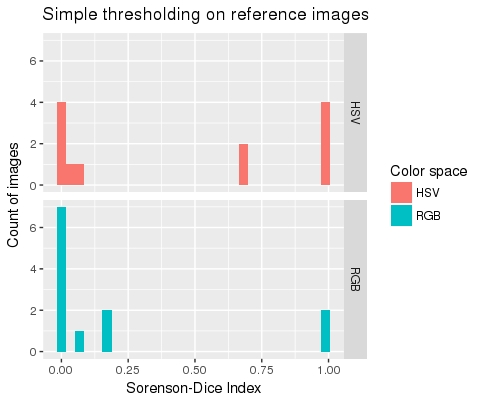
\includegraphics[width=\linewidth]{images/simple_ref.jpeg}
    \caption{Distribution of evaluation results for simple thresholding in two color spaces on reference images.}
    \label{fig:simple-ref}
\end{figure}

% histogram for simple thresholding customer images
\begin{figure}
    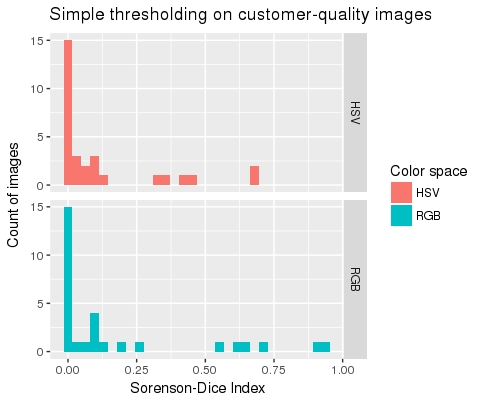
\includegraphics[width=\linewidth]{images/simple_cust.jpeg}
    \caption{Distribution of evaluation results for simple thresholding in two color spaces on customer-quality images.}
    \label{fig:simple-cust}
\end{figure}

\subsubsection{Distance to average}

We perform thresholding on distance to average on reference images using both mean and median as measures of the average in both RGB and HSV space. Thresholding using mean in RGB space gives a mean Sorenson-Dice index of .652 with 50\% of images over .9 and the remaining 50\% under .5. Thresholding using mean in HSV space gives a mean Sorenson-Dice index of .629 with 50\% of images over .9 and the remaining 50\% under .5. Thresholding using median in RGB space gives a mean Sorenson-Dice index of .991 with 100\% of images over .9. Thresholding using median in HSV also gives a mean Sorenson-Dice index of .992 with 100\% of images over .9, as shown in Figure \ref{fig:dist-thresh}. For customer-quality images, thresholding using median in RGB space gives a mean Sorenson-Dice index of .051 with no images over .5. Thresholding using median in HSV space on customer-quality images gives a mean Sorensen-Dice index of .052 with no images over .5. Thresholding using mean in RGB space on customer-quality images gives a mean Sorenson-Dice index of .089 with no images over .9 and 3.3\% of images over .5. Thresholding using mean gives a mean Sorenson-Dice index of .091 with no images over .5.

% histogram for distance thresholding
\begin{figure}
    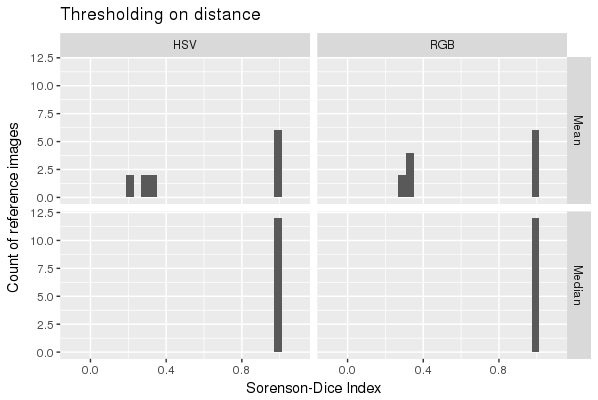
\includegraphics[width=\linewidth]{images/dist_gray.jpeg}
    \caption{Distribution of evaluation results for thresholding on the distance to the mean versus median color and RGB versus HSV color space.}
    \label{fig:dist-thresh}
\end{figure}

\subsubsection{Watershed Algorithm}

We perform the Watershed Algorithm \cite{watershed} on reference and customer-quality images in both HSV and RGB space, as shown in Figure \ref{fig:water}. Watershed on reference images in RGB space gives a mean Sorenson-Dice index of .817 with 75\% of images above .9 and the remaining images under .5. Watershed on reference images in HSV space gives a mean Sorenson-Dice index of .525 with 16.7\% of images above .9 and 50\% of images above .5. Watershed on customer-quality images in RGB space gives a mean Sorenson-Dice index of .180 with 3.3\% of images above .9 and 16.7\% of images above .5. Watershed on customer-quality images in HSV space gives a mean Sorenson-Dice index of .242 with 10\% of images above .9 and 23.3\% of images above .5.

% histogram for water
\begin{figure}
    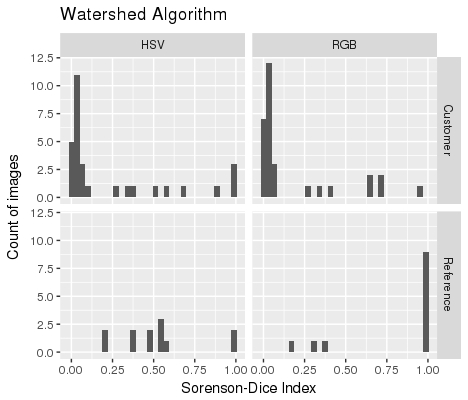
\includegraphics[width=\linewidth]{images/water.jpeg}
    \caption{Distribution of evaluation results for the Watershed Algorithm on reference versus customer-quality images and RGB versus HSV color spaces.}
    \label{fig:water}
\end{figure}

\subsection{Discussion}
\label{discussion}

We find that none of the image segmentation techniques we compare are consistently effective for customer-quality images, but thresholding on distance to median is very effective for segmenting reference-quality images, and some select images are accurately segmented with other methods.

Simple thresholding is generally ineffective, especially on customer-quality images. Many of these images have hard shadows or other variations in background color or hue such that simple thresholding isolates these regions instead of isolating the pill; this is particularly prevalent when the pill is a similar color to the unshadowed background, see Figure \ref{fig:bad-simple-hsv}. We find in some cases simple thresholding performs better in HSV space than RGB space, as shown when comparing Figures \ref{fig:ok-simple-hsv} and \ref{fig:ok-simple-rgb}. This is because the background is not a consistent color, but it does have a consistent \textit{hue} (in this case, the background is also the same hue as half of the pill). Additionally, simple thresholding does successfully segment several reference images of single-color pills that are very different from their backgrounds, as in Figure \ref{fig:good-simple-hsv}.

% bad customer quality HSV simple
\begin{figure}
    
\includegraphics[width=\linewidth]{images/simple_hsv_bad.jpg}
    \caption{Simple threshodling in HSV space did not perform well on this image. Left: simple thresholding output. Center: original image. Right: hand-segmented binary image.}
    \label{fig:bad-simple-hsv}
\end{figure}

% simple HSV relative success
\begin{figure}
    
\includegraphics[width=\linewidth]{images/simple_hsv_ok.jpg}
    \caption{Simple thresholding in HSV, pictured here, performed better (but not perfectly) on this image than in RGB space, pictured in Figure \ref{fig:ok-simple-rgb}. Left: simple thresholding output. Center: original image. Right: hand-segmented binary image.}
    \label{fig:ok-simple-hsv}
\end{figure}

% comparing above to simple RGB
\begin{figure}
    
\includegraphics[width=\linewidth]{images/simple_rgb_ok.jpg}
    \caption{Simple thresholding in HSV, pictured in Figure \ref{fig:ok-simple-hsv}, performed better on this image than in RGB space, pictured here. Note that the bottom of the image is white. Left: simple thresholding output. Center: original image. Right: hand-segmented binary image.}
    \label{fig:ok-simple-rgb}
\end{figure}

% good reference quality HSV simple
\begin{figure}
    
\includegraphics[width=\linewidth]{images/simple_hsv_good.jpg}
    \caption{Simple thresholding in HSV space performed well on this image. Left: simple thresholding output. Center: original image. Right: hand-segmented binary image.}
    \label{fig:good-simple-hsv}
\end{figure}

Thresholding on distance to average is very effective on reference images, especially using the median as the measure of average, as shown in Figure \ref{fig:dist-med-compare}. This is effective because the majority of each reference image is the gray of the background; thresholding on the median isolates this color. Thresholding on the mean is nowhere near as effective as thresholding on the distance from the median, as shown in Figure \ref{fig:dist-mean-compare}, because the median is more resistant to outliers than the mean and therefore more reliably identifies the background gray. However, because the customer-quality images do not have consistent backgrounds like the reference images, this method is not at all effective for customer-quality images with mean or median in either color space. 

% distance from median thresholding
\begin{figure}
    
\includegraphics[width=\linewidth]{images/dist_med_compare.jpg}
    \caption{Thresholding on the distance from the median is effective on all reference images (as shown here), unlike thresholding on the distance from the mean as shown in Figure \ref{fig:dist-mean-compare}. Left: thresholding output. Center: original image. Right: hand-segmented binary image.}
    \label{fig:dist-med-compare}
\end{figure}

% distance from mean thresholding
\begin{figure}
    
\includegraphics[width=\linewidth]{images/dist_mean_compare.jpg}
    \caption{Thresholding on the distance from the median is effective on all reference images as shown in Figure \ref{fig:dist-med-compare}, unlike thresholding on the distance from the mean as shown here. Left: thresholding output, clearly ineffective. Center: original image. Right: hand-segmented binary image.}
    \label{fig:dist-mean-compare}
\end{figure}

Watershed is generally not very effective, although it performs relatively well on reference-quality images in RGB space. Unlike simple thresholding, Watershed gives better results for RGB space than HSV space for reference-quality images, as shown in Figures \ref{fig:water-ref-hsv} and \ref{fig:water-ref-rgb}. Watershed is very effective for a few customer-quality images in HSV space featuring orange pills on gray backgrounds, although Watershed does not effectively segment these images in RGB space, as shown in Figures \ref{fig:water-cust-rgb} and \ref{fig:water-cust-hsv}.

% watershed reference in RGB
\begin{figure}
    
\includegraphics[width=\linewidth]{images/water_ref_rgb.jpg}
    \caption{The Watershed Algorithm is effective for some reference images in RGB space, as shown here, but not in HSV space, as shown in Figure \ref{fig:water-ref-hsv}. Left: Watershed output. Center: original image. Right: hand-segmented binary image.}
    \label{fig:water-ref-rgb}
\end{figure}

% watershed reference in HSV
\begin{figure}
    
\includegraphics[width=\linewidth]{images/water_ref_hsv.jpg}
    \caption{The Watershed Algorithm is effective for some reference images in RGB space, as shown in Figure \ref{fig:water-ref-rgb}, but not in HSV space, as shown here. Left: Watershed output. Center: original image. Right: hand-segmented binary image.}
    \label{fig:water-ref-hsv}
\end{figure}

% watershed customer in RGB
\begin{figure}
    
\includegraphics[width=\linewidth]{images/water_cust_rgb.jpg}
    \caption{Watershed is more effective for a few customer-quality images in HSV space, shown in Figure \ref{fig:water-cust-hsv}, than in RGB space, shown here. Left: Watershed output. Center: original image. Right: hand-segmented binary image.}
    \label{fig:water-cust-rgb}
\end{figure}

% watershed customer in HSV
\begin{figure}
    
\includegraphics[width=\linewidth]{images/water_cust_hsv.jpg}
    \caption{Watershed is more effective for a few customer-quality images in HSV space, shown here, than in RGB space, shown in Figure \ref{fig:water-cust-rgb}. Left: Watershed output. Center: original image. Right: hand-segmented binary image.}
    \label{fig:water-cust-hsv}
\end{figure}

For some images, especially reference images, the Sorenson-Dice index is higher than expected looking at the actual segmented image. For example, the segmented image in Figure \ref{fig:dist-mean-compare} is completely white, but it gives a Sorenson-Dice index of .281 because the Sorenson-Dice index penalizes false positives less than false negatives. This seems artificially high, so there may exist a more precise metric of segmentation comparison than we use here. However, the Sorenson-Dice index does accurately represent good segmentations, so it fulfills our purposes well enough. 

Overall, thresholding on distance to median gives the best results, but only on reference images. Watershed also gives decent results for reference images in RGB space, but not with the consistency of thresholding on the median. Simple thresholding also accurately segments some reference images, but is again not as consistent as thresholding on the median. However, thresholding on the median is extremely ineffective for customer-quality images. Watershed accurately segments several customer-quality images, but does not succeed at segmenting the majority of customer-quality images. Similarly, simple thresholding is slightly effective on a few customer-quality images, but these are exceptions. Generally, we are not able to segment customer-quality images, although we are able to consistently and accurately segment reference images.

\section{Conclusions}
\label{conclusions}

The NLM’s Pill Image Recognition Challenge presents both an important and difficult task to the bioinformatics and computer vision communities. We aim to work on the important pre-processing step of isolating pills within the images in the PIll Image Recognition Challenge dataset. We explore several techniques for segmenting both the higher quality reference images, with consistent background colors and no harsh shadows, and the customer-quality images, with inconsistent backgrounds, photography angles, and lighting conditions. While no technique gives consistently good results in segmenting the customer-quality images, thresholding on the distance from the median pixel color gives consistently accurate results in segmenting reference images; the Sorensen-Dice Indices are above .97 for all the reference images for which we have manually segmented counterparts. Several other techniques give decent results on non-white solid-colored reference images, but none comes close the technique of thresholding on the distance from the median (or even from the mean, the results for which are less consistent). We successfully segment several of the customer-quality images but no technique results in consistently good segmentations even within a category of pills (e.g. white pills, non-white solid-colored pills) for customer-quality images. 

Because none of our techniques consistently provides useful segmentations for customer-quality images, this remains an important area for future work. While this likely requires many more manually segmented images, we would like to try training a convolutional neural net. Dave and Matt Zucker have had success with this technique for segmenting images  of flies and classifying image regions as body parts \cite{mattzraps}. Our application has less consistent image backgrounds than the fly sorter, but has analogous issues with shadows, and is likely less complicated than fly classification in terms of the angles of the images and the complexity of the required segmentation. We are therefore hopeful that this technique will provide consistent and accurate results on our dataset. 

Marker-Controlled Watershed algorithms could also possibly give better results on customer-quality images \cite{image-seg}. Our Watershed technique identifies markers heuristically, while Marker-Controlled Watershed performs the flooding algorithm from inputted keypoints. With this algorithm, we would have more control over which regions are selected and therefore not have to rely on position in the image file as a means of selecting the region corresponding with the pill. We hypothesize that this technique would improve the results of the Watershed Algorithm applied to customer-quality images, but it would require user input to seed the program with a keypoint inside the pill in each image. Unfortunately, this may also make any tool resulting from this work less accessible to those with visual impairments, nullifying an important part of its purpose. 

Another area of research we hope to pursue is using K-mean clustering for image segmentation as well as for classification.  K-means for image segmentation is a promising technique that we begin exploring in our source code.  However, it is non-trivial to determine the correct number of clusters to use with the algorithm, as is often the case with k-means. The algorithm also does not result in a binary segmentation and it is therefore difficult to determine which region of the segmentation should be considered the foreground when converting to a binary mask. We believe some of these challenges can be addressed by considering the shape of the regions - perhaps building on the work of Ushizima et al. to match segmentation regions to identifiable pill shapes. 

K-means may also be useful as a means of creating features with which to learn a distance function between the reference images and the customer-quality images.  We hypothesize that creating feature vectors with the means of pixel-color clusters and the proportion of the image that belongs to each could be simple but effective as input to Large Margin Nearest Neighbor or a related algorithm. 

We successfully segment reference images, and aim to use Marker-Controlled Watershed algorithms, and convolutional neural networks to improve our segmentation for customer-quality images in the future. Additionally, we plan to move past segmentation to actual pill classification, possibly using k-means with distance learning or further convolutional neural networks. With further work, pill classification can be faster, more convenient, and more accurate for those who must frequently identify pills by sight, leading to fewer dangerous mishaps regarding misidentified pills.

\section*{Acknowledgments}

We would like to thank Professor Ameet Soni for all of his support and assistance. We would also like to thank Professor Matt Zucker for giving computer vision advice and resources. Finally, we would like to thank researchers Ushizima et al. for sharing the full text of their paper on ResearchGate only a few hours after we requested it.

% also thanks to Oberon for being growly and silly and a good dog

% In the unusual situation where you want a paper to appear in the
% references without citing it in the main text, use \nocite
\nocite{ushizima}
\nocite{PIR}

\bibliography{references}
\bibliographystyle{icml2014}

\end{document}


% This document was modified from the file originally made available by
% Pat Langley and Andrea Danyluk for ICML-2K. This version was
% created by Lise Getoor and Tobias Scheffer, it was slightly modified
% from the 2010 version by Thorsten Joachims & Johannes Fuernkranz,
% slightly modified from the 2009 version by Kiri Wagstaff and
% Sam Roweis's 2008 version, which is slightly modified from
% Prasad Tadepalli's 2007 version which is a lightly
% changed version of the previous year's version by Andrew Moore,
% which was in turn edited from those of Kristian Kersting and
% Codrina Lauth. Alex Smola contributed to the algorithmic style files.
